%-*- coding:utf-8 -*-

\documentclass[dvipdfmx]{beamer}
\usepackage{tutorial}

\title{計算機実験II (L2) --- モンテカルロと統計力学}
\date{2019/10/18}

\begin{document}

\begin{frame}
  \titlepage
  \tableofcontents
\end{frame}

\section{多体系の統計力学}

\begin{frame}[t,fragile]{典型的な統計力学モデル}
  \begin{itemize}
    %\setlength{\itemsep}{1em}
  \item 古典粒子系
    \begin{itemize}
    \item 調和振動子 \ \ $\displaystyle H = \frac{p^2}{2m} + \frac{k}{2}x^2$
    \item 多粒子系
      \[
      H = \sum \frac{p_i^2}{2m} + \sum_{ij} V(x_i, x_j)
      \]
    \item バネビーズ模型
      \[
      H = \sum \frac{p_i^2}{2m} + \frac{k}{2} \sum_{ij} (x_i-x_j)^2
      \]
  \end{itemize}
  \item 磁性体
    \begin{itemize}
    \item イジング模型 \ \ $\displaystyle H = -J \sum_{ij} \sigma_i \sigma_j$ \ \ \ $\sigma_i = \pm 1$
    \end{itemize}
  \end{itemize}
\end{frame}

%-*- coding:utf-8 -*-

\begin{frame}[t,fragile]{多体系の統計力学}
  \begin{itemize}
    %\setlength{\itemsep}{1em}
  \item カノニカル分布 \ $\pi(s) = \exp [- \beta H(s) ] / Z$ \ \ \ ($\beta = k_{\rm B} T$)
  \item 分配関数・自由エネルギー
    \begin{align*}
      Z(T) &= \int \exp [- \beta H(p,x) ] \, dp \, dx \qquad \text{(連続変数)} \\
      &= \sum_s \exp [- \beta H(s) ] \qquad \text{(離散変数)} \\
      f(T) &= - \beta^{-1} \log Z(T)
    \end{align*}
  \item 物理量の期待値
    \begin{align*}
      \langle A \rangle &= Z^{-1} \int A(p,x) \exp [- \beta H(p,x) ] \, dp \, dx \qquad \text{(連続変数)} \\
      &= Z^{-1} \sum_s A(s) \exp [- \beta H(s) ] \qquad \text{(離散変数)}
    \end{align*}
  \end{itemize}
\end{frame}

%-*- coding:utf-8 -*-

\begin{frame}[t,fragile]{多体系の統計力学}
  \begin{itemize}
    % \setlength{\itemsep}{1em}
  \item 内部エネルギー
    \begin{align*}
      E &= -\frac{\partial}{\partial\beta} \log Z = Z^{-1} \sum_s H(s) \exp [- \beta H(s) ] = \langle H \rangle
    \end{align*}
  \item 比熱
    \begin{align*}
      C &= \frac{1}{N} \frac{\partial E}{\partial T} = \frac{\beta^2}{N} (\langle H^2 \rangle - \langle H \rangle^2)
    \end{align*}
  \end{itemize}
\end{frame}

%-*- coding:utf-8 -*-

\begin{frame}[t,fragile]{様々な数値計算手法}
  \begin{itemize}
    % \setlength{\itemsep}{1em}
  \item 数え上げ (離散変数)
    \begin{itemize}
      \item 計算コスト × (指数関数的)
      \item メモリコスト ○ (${\cal O}(1)$)
    \end{itemize}
  \item 転送行列法 (離散変数)
    \begin{itemize}
      \item 計算コスト △ (指数関数的)
      \item メモリコスト △ (指数関数的)
    \end{itemize}
  \item 分子動力学法 (連続変数)
    \begin{itemize}
      \item 計算コスト ○ (${\cal O}(N)$)
      \item メモリコスト ○ (${\cal O}(N)$)
      \item 統計誤差あり
    \end{itemize}
  \item マルコフ連鎖モンテカルロ法 (離散変数・連続変数)
    \begin{itemize}
      \item 計算コスト ○ (${\cal O}(N)$)
      \item メモリコスト ○ (${\cal O}(N)$)
      \item 統計誤差あり
    \end{itemize}
  \end{itemize}
\end{frame}


\section{乱択アルゴリズム}
\begin{frame}[t,fragile]{乱択アルゴリズム(randomized algorithm)}
  \begin{itemize}
    %\setlength{\itemsep}{1em}
  \item 実行中に乱数を参照してその値によって振る舞いをかえるアルゴリズム
  \item ラスベガスアルゴリズム
    \begin{itemize}
    \item 乱数の出方によらず常に正しい結果を与えるアルゴリズム
    \item 平均化効果を利用するアルゴリズム:クイックソート
    \end{itemize}
  \item モンテカルロアルゴリズム
    \begin{itemize}
    \item 乱数の出方によっては誤った結果を与えるアルゴリズム
    \item 標本を利用するアルゴリズム:最大カット問題
    \item くじ引き型のアルゴリズム:素数性判定、関数の同一性、行列積の検算
    \item サンプリングアルゴリズム:モンテカルロ積分、マルコフ連鎖モンテカルロ
    \end{itemize}
  \end{itemize}
\end{frame}

\begin{frame}[t,fragile]{乱択クイックソート}
  \begin{itemize}
    %\setlength{\itemsep}{1em}
  \item 分割統治法に基づく再帰的なソートアルゴリズム
    \begin{itemize}
      \item 配列の中から要素を一つ選び、それより小さい要素からのみなる集合と大きい要素のみからなる集合の2つに分ける
      \item それぞれの集合をソートし、結合する
    \end{itemize}
    \item ほぼ同じ大きさの集合に分けることができる場合の実行ステップ数$\sim {\cal O}(n \log n)$
    \item 最悪(選んだ要素が常に最大 or 最小値)の場合のステップ数$\sim {\cal O}(n^2)$
    \item 分割に用いる要素を「ランダムに」選ぶ $\Rightarrow$ 平均ステップ数$\sim {\cal O}(n \log n)$
  \end{itemize}
\end{frame}

\begin{frame}[t,fragile]{クイックソート}
  \resizebox{!}{.7\textheight}{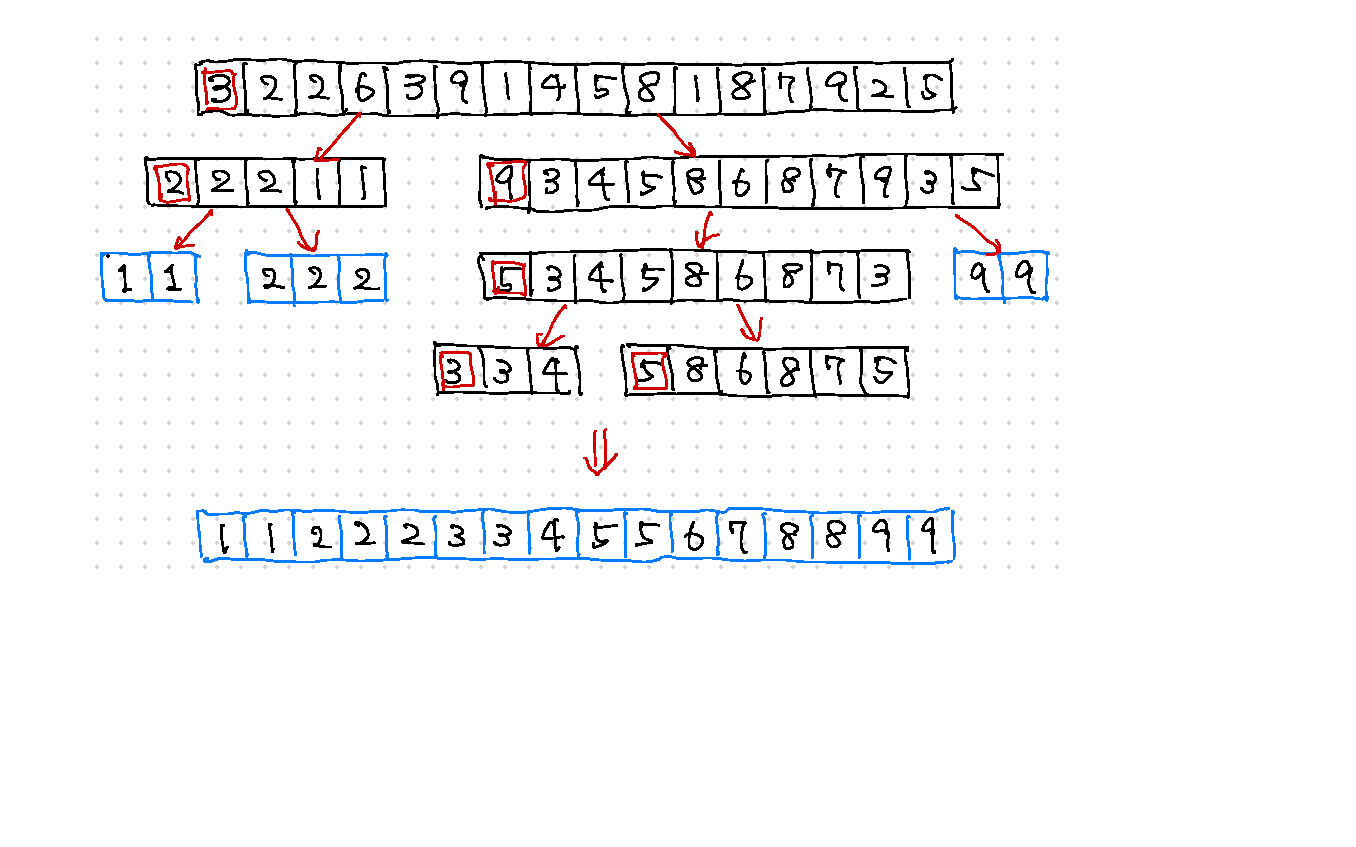
\includegraphics{image/quicksort.pdf}}
\end{frame}


\section{物理過程のシミュレーション}

\begin{frame}[t,fragile]{物質中の中性子輸送}
  \begin{center}
  \resizebox{0.45\textwidth}{!}{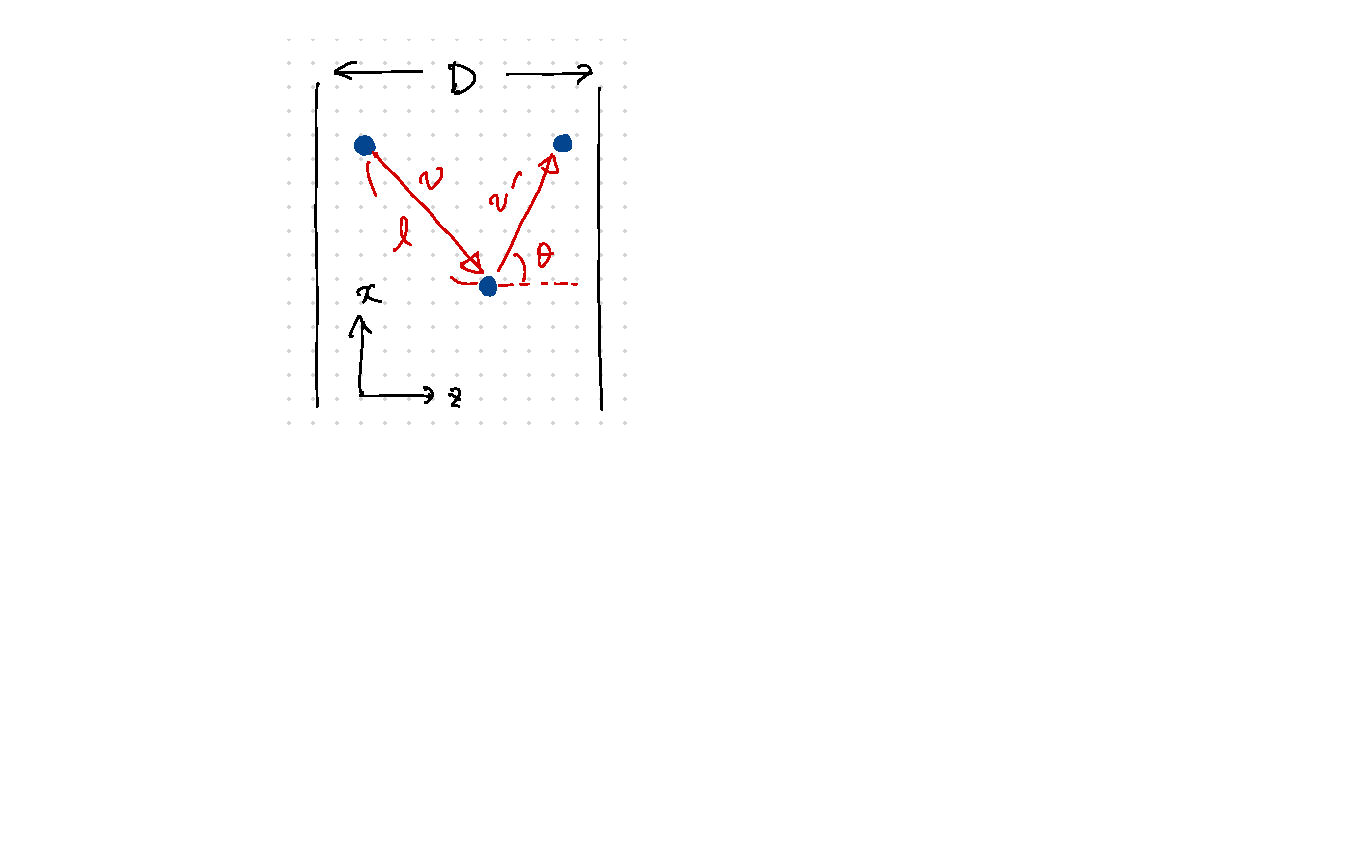
\includegraphics{image/scattering.pdf}}
  \end{center}
\end{frame}

\begin{frame}[t,fragile]{物質中の中性子輸送}
  \begin{itemize}
    %\setlength{\itemsep}{1em}
  \item ある板状の物質(厚さ$D$)に垂直に中性子が入射したときの吸収率・透過率・反射率
  \item 中性子はある確率で物質の原子核に衝突し、確率$p_{\rm c}$で吸収、$p_{\rm s}=1-p_{\rm c}$で散乱される
    \begin{itemize}
    \item 衝突は確率的に起きるので、次の衝突までの距離$\ell$は指数分布にしたがう($\lambda^{-1}$: 平均自由行程)
      \[
      p(\ell) = \lambda e^{-\lambda\ell}
      \]
    \item 衝突時、ランダムな方向に散乱されるとすると
      \[
      p(\theta,\phi) \, d\theta \, d\phi = \frac{d\Omega}{4\pi} = \frac{\sin \theta}{4\pi} \, d\theta \, d\phi
      \]
      \[
      p(\theta) = \frac{\sin \theta}{2} \qquad p(\phi)=\frac{1}{2\pi}
      \]
    \end{itemize}
  \end{itemize}
\end{frame}

\begin{frame}[t,fragile]{モンテカルロシミュレーション}
  \begin{enumerate}
    %\setlength{\itemsep}{1em}
  \item 初期条件 $z=0$, $\theta = 0$
  \item {\color{red} 指数分布から$\ell$を選ぶ}
  \item $z \leftarrow z + \ell \cos \theta$
  \item $z<0$ → 反射(終了) \\
    $z>D$ → 透過(終了) \\
    $0 < z < D$ → 確率$p_{\rm c}$で吸収(終了)、$p_{\rm s}$で散乱
  \item {\color{red} 散乱後の$\theta$を選び}、2に戻る
  \end{enumerate}
  \vspace*{-3.5cm}\hspace{8cm}\resizebox{0.25\textwidth}{!}{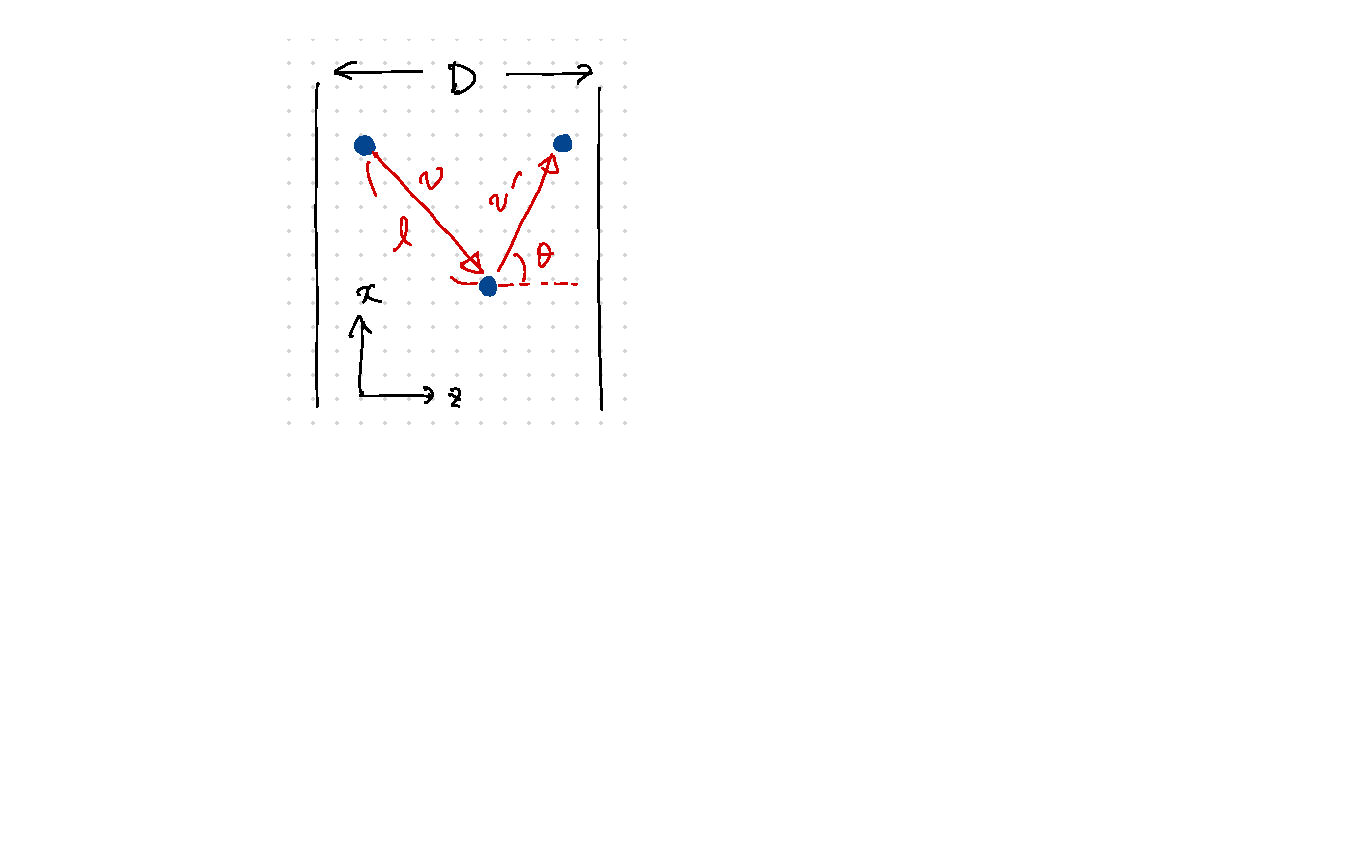
\includegraphics{image/scattering.pdf}}
\end{frame}


\section{擬似乱数}

\begin{frame}[t,fragile]{乱数}
  \begin{itemize}
    \setlength{\itemsep}{1em}
  \item 自然乱数 (ハードウェア乱数)
    \begin{itemize}
    \item さいころ, コイン, ルーレット, 核分裂反応, 熱雑音, ショット雑音 ...
    \end{itemize}
  \item モンテカルロシミュレーションにおける必要条件
    \begin{itemize}
    \item 多数の乱数が必要
    \item ポータビリティ
    \item 生成速度
    \item 再現性
    \end{itemize}
  \item 擬似乱数 (pseudo random number)
    \begin{itemize}
    \item 計算機でプログラムに従って生成
    \item 分布の一様性, 相関, 周期に注意する必要あり
    \end{itemize}
  \end{itemize}
\end{frame}

\begin{frame}[t,fragile]{擬似乱数発生器}
  \begin{itemize}
    %\setlength{\itemsep}{1em}
  \item 最も簡単な乱数発生器:線形合同法 (linear congruential method)
    \[
    x_{n+1} = (ax_n+c) \ \mbox{mod} \ m
    \]
  \item 例) $a = 65539$, $c = 0$, $m = 2147483648$ (周期 $m-1$)
  \item 少しだけ異なる初期値 $(x0 = 1, 2, 3)$ から始めた場合
  \resizebox{!}{.35\textheight}{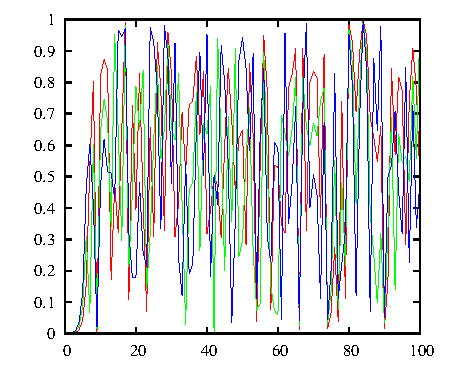
\includegraphics{image/lcg-1.pdf}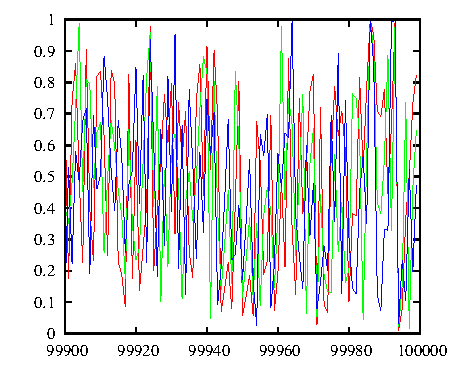
\includegraphics{image/lcg-2.pdf}}
  \item 数十ステップ進むとバラバラな振舞い ⇒ カオス的
  \end{itemize}
\end{frame}

\begin{frame}[t,fragile]{擬似乱数生成器における相関}
  \begin{itemize}
    %\setlength{\itemsep}{1em}
  \item 合同乗算法で多次元超立方体中に「ランダムに」点を打つと、それらの点は全て比較的小数の等間隔に並んだ超平面の上にのってしまう (多次元疎結晶構造)
  \resizebox{!}{.35\textheight}{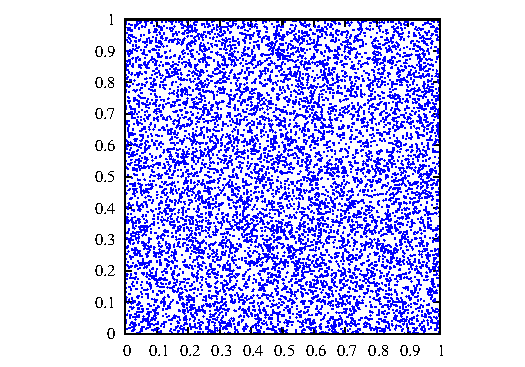
\includegraphics{image/lcg-2d.pdf}}
  \resizebox{!}{.35\textheight}{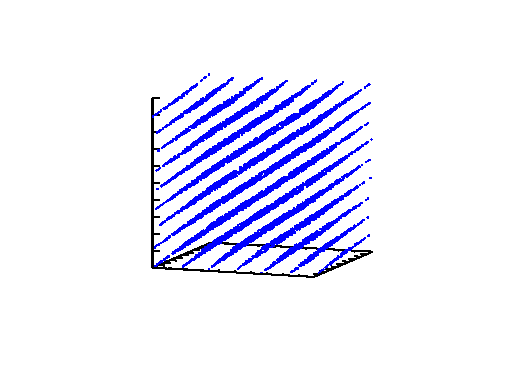
\includegraphics{image/lcg-3d.pdf}}
  \item 計算式に従って生成するため、必ず何らかの相関は残る
  \item できる限り相関が少なく周期の長い、理想的な乱数の開発が続けられている
    \begin{itemize}
    \item 現時点で、標準的な乱数発生器:メルセンヌ・ツイスター
    \item 周期 $2^{19937}-1$、高速、日本製! (例: \href{https://github.com/todo-group/computer-experiments/blob/master/exercise/monte_carlo/random.c}{example-2-L2/random.c})
    \end{itemize}
  \end{itemize}
\end{frame}

\begin{frame}[t,fragile]{乱数発生器の選び方}
  \begin{itemize}
    %\setlength{\itemsep}{1em}
  \item 万能乱数発生器は存在しない
  \item 生成された乱数のもつ性質について, 様々な数学的に厳密な証明, 多くのテスト結果がすでに存在するが, 特定のシミュレーションに使った場合の結果については何も保証してくれない
  \item 自分で乱数発生器を「発明」してはいけない
  \item 自分で乱数発生器をプログラムしてはいけない (既存のライブラリを使う)
  \item 初期化(種の設定)を正しく行う
  \item 実際にそれらしい乱数が生成されているか, 目でみて確認する
  \item 二種類以上の乱数発生器を使ってみて, 互いに一致する結果が出るかどうか確認する
  \end{itemize}
\end{frame}

\begin{frame}[t,fragile]{様々な分布}
  \begin{itemize}
    %\setlength{\itemsep}{1em}
  \item 乱数発生器は通常、一様な整数乱数あるいは実数乱数を生成
  \item 一様分布以外の分布にしたがう乱数の発生方法の代表例
  \item 逆関数法
    \begin{itemize}
      \item 確率分布関数$F(x)$の逆関数$F^{-1}(y)$ と(0,1)の一様乱数$u$から $v=F^{-1}(u)$
      \item 例: 指数分布 $p(x) = \frac{1}{\mu} e^{-x/\mu}$

      $F(x) = 1 - e^{-x/\mu}$ \ \ \ $F^{-1}(y) = - \mu \log(1-y)$
      \item 一般の確率分布関数について逆関数を求めるのは困難
    \end{itemize}
  \item 棄却法
    \begin{itemize}
      \item 確率密度関数を完全に囲むような箱を用意し、その箱の中で一様乱数を生成
      \item 確率密度関数の下側の点が生成されたら、その$x$座標を乱数として採用。上側の点の場合には再度生成
      \item もとの確率密度関数よりも箱が大きくなりすぎると非効率
    \end{itemize}
  \end{itemize}
\end{frame}

% -*- coding: utf-8 -*-

\documentclass[10pt,dvipdfmx]{beamer}
\usepackage{tutorial}

\begin{document}
\section{ヒストグラム}
\begin{frame}[t,fragile]{疑似乱数とは}
  \begin{itemize}
    %\setlength{\itemsep}{1em}
  \item 計算機でプログラムに従って生成する乱数(のようなもの)
  \item 乱数は何に役立つか?
    \begin{itemize}
    \item 等式のチェック、例外の発見
    \item 初期値にランダムネスを入れることで最悪の場合を避ける
    \item サンプリングを使ったシミュレーション (→計算機実験II)
    \end{itemize}
  \item 乱数を使う場合の注意
    \begin{itemize}
    \item 計算式に従って生成するため周期は有限であり、必ず何らかの相関がある
    \item 初期化(種の設定)を正しく行う
    \item 実際にそれらしい乱数が生成されているか目で見て確認する
    \end{itemize}
  \item 代表的な乱数発生器のひとつ: メルセンヌ・ツイスター
    \begin{itemize}
    \item 周期 $2^{19937}-1$、高速、日本製!
    \item ヘッダファイル: \href{https://github.com/todo-group/computer-experiments/blob/master/exercise/monte_carlo/mersenne_twister.h}{mersenne\_twister.h}
    \item サンプルプログラム: \href{https://github.com/todo-group/computer-experiments/blob/master/exercise/monte_carlo/random.c}{random.c}
    \end{itemize}
  \end{itemize}
\end{frame}

\begin{frame}[t,fragile]{様々な分布}
  \begin{itemize}
    %\setlength{\itemsep}{1em}
  \item 乱数発生器は通常、一様な整数乱数あるいは実数乱数を生成
  \item 一様分布以外の分布にしたがう乱数の発生方法の代表例
  \item 逆関数法
    \begin{itemize}
      \item 確率分布関数$F(x)$の逆関数$F^{-1}(y)$ と(0,1)の一様乱数$u$から $v=F^{-1}(u)$
      \item 例: 指数分布 $p(x) = \frac{1}{\mu} e^{-x/\mu}$

      $F(x) = 1 - e^{-x/\mu}$ \ \ \ $F^{-1}(y) = - \mu \log(1-y)$
      \item 一般の確率分布関数について逆関数を求めるのは困難
    \end{itemize}
  \item 棄却法
    \begin{itemize}
      \item 確率密度関数を完全に囲むような箱を用意し、その箱の中で一様乱数を生成
      \item 確率密度関数の下側の点が生成されたら、その$x$座標を乱数として採用。上側の点の場合には再度生成
      \item もとの確率密度関数よりも箱が大きくなりすぎると非効率
    \end{itemize}
  \end{itemize}
\end{frame}

\begin{frame}[t,fragile]{ヒストグラムの作り方}
  \begin{itemize}
    %\setlength{\itemsep}{1em}
  \item 連続変数(実数)のデータの場合 ([]内はサンプルプログラムでの変数名)
    \begin{itemize}
    \item $N$: サンプル数 [{\tt samples}]
    \item $x_{\rm min}$: データの最小値(カットオフ) [{\tt xmin}]
    \item $x_{\rm max}$: データの最大値(カットオフ) [{\tt xmax}]
    \item $n$: ビンの個数 [{\tt bins}]
    \item $\Delta$: ビンの幅 ($\Delta=(x_{\rm max}-x_{\rm min}) / n$) [{\tt dx}]
    \end{itemize}
  \item サイズ$n$の配列を準備
    \begin{itemize}
    \item データ毎にどのビンに入るか計算: $j = (x - x_{\rm min}) / \Delta$
    \item (必要に応じて) $0 \le j < n$であることを確認 (範囲外のデータは無視する)
    \item 配列の$j$番目の値を1増やす
    \end{itemize}
  \item サンプルプログラム: \href{https://github.com/todo-group/computer-experiments/blob/master/exercise/monte_carlo/histogram.c}{histogram.c}

    (コンパイルには\href{https://github.com/todo-group/computer-experiments/blob/master/exercise/include/mersenne_twister.h}{mersenne\_twister.h}と\href{https://github.com/todo-group/computer-experiments/blob/master/exercise/include/cmatrix.h}{cmatrix.h}が必要)
  \end{itemize}
  \vspace*{-5.5cm} \hfill \resizebox{0.28\textwidth}{!}{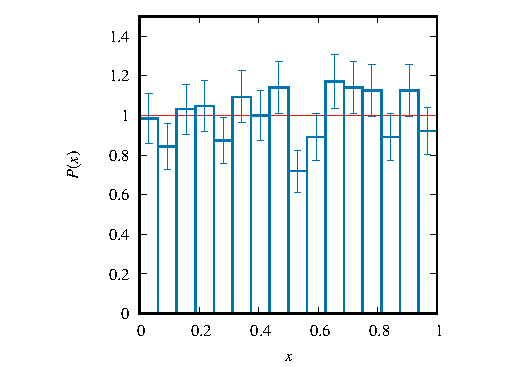
\includegraphics{image/histogram.pdf}}
\end{frame}

\begin{frame}[t,fragile]{ビンの個数の設定}
  \begin{itemize}
  \item 最適の幅というものはない
  \item 個数を増やすと表現の自由度は増えるが、各ビンのエラーバーが大きくなる
    \begin{itemize}
    \item データが統計的に独立である場合、それぞれのビンのカウント数$m$はポワソン分布に従う
    \item 統計誤差 $\sim \sqrt{m}$
    \end{itemize}
  \item いくつかの方法・公式が提案されているが、分布の形によっては不適切な場合も
    \begin{itemize}
    \item スタージェスの公式 $n = \log_2 N + 1$
    \item スコットの公式 $\Delta = 3.5 \sigma / N^{1/3}$
    \end{itemize}
  \item 実際には、ビンの個数を何通りか試してみるのが良い
  \item データを取り直すことが出来ない and/or コストがかかる場合も多いので、生データはいったんファイルに保存しておく
  \end{itemize}
\end{frame}

\end{document}

\section{モンテカルロ積分}

\begin{frame}[t,fragile]{モンテカルロ積分}
  \begin{itemize}
    \setlength{\itemsep}{1em}
  \item 円周率を与える公式
    \[
    \pi = \lim_{c \rightarrow \infty} \int_0^c f(x) \, dx \ \ \ f(x) = \frac{2}{\cosh x}
    \]
  \item スタンダードな数値積分法: 台形公式 (一次式補間), シンプソン公式 (二次式補間), etc
  \item カットオフ $c$ の値
    \begin{itemize}
    \item 誤差は $c$ が大きくなると指数関数的に小さくなる
    \item 例えば $c = 20$ で誤差は $8.3 \times 10^{-9}$ 以下
    \end{itemize}
  \end{itemize}
\end{frame}

\begin{frame}[t,fragile]{単純サンプリング}
  \begin{itemize}
    \setlength{\itemsep}{1em}
  \item $[0,c]$ と $[0,2]$ の一様分布から二次元上の点 $(x,y)$ を $M$ 組生成
  \item $f(x)$ の下に入った数 $N$ をカウント
    \[
    \pi \simeq 2c \times \frac{N}{M}
    \]
    \begin{tabular}{|c|c|c|}
      \hline
      $M$ & 平均値 & 誤差 \\
      \hline
      100 & 4.8 & 1.3 \\
      10000 & 3.12 & 0.11 \\
      1000000 & 3.154 & 0.011 \\
      \hline
    \end{tabular}
  \end{itemize}
  \vspace*{-7em}
  \hspace*{17em}
  \resizebox{!}{.45\textheight}{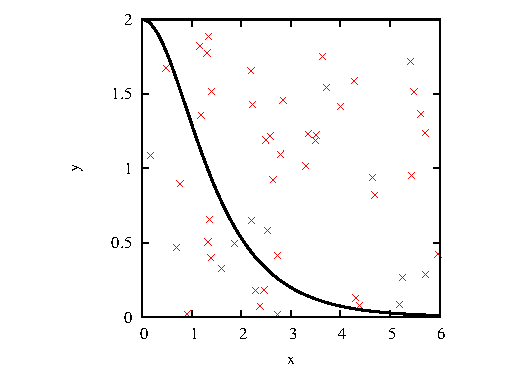
\includegraphics{image/coth-1.pdf}}
\end{frame}

\begin{frame}[t,fragile]{統計誤差の評価}
  \begin{itemize}
    \setlength{\itemsep}{1em}
  \item このモンテカルロ積分が実際に評価している積分
    \[
    \frac{1}{2c} \int_0^c \!\! \int_0^2 \!\! \theta(x,y) \, dx \, dy
    \ \ \ \theta(x,y) = \begin{cases} 2c & \text{if $y < f(x)$} \\ 0 & \text{otherwise} \end{cases}
    \]
  \item 統計誤差の評価
    \begin{itemize}
      \item 試行の成功確率(success probability): $q=\frac{\pi}{2c}$
      \item 一回の試行の平均値(mean): $\mu = 2c \times q = \pi$
      \item 分散(variance):
        \[ s^2 = (2c)^2q + 0^2(1-q) - \mu^2 = 2c\pi-\pi^2 = 4c^2 q(1-q) \]
      \item $c=20$ の時:
        \[ q \simeq 0.0785 \ \ \ s^2 \simeq 116
        \]
    \end{itemize}
  \end{itemize}
\end{frame}

\begin{frame}[t,fragile]{中心極限定理(central limiting theorem)}
  \begin{itemize}
    %\setlength{\itemsep}{1em}
  \item $M$回の試行のうち $N$回成功する確率 ($\pi$の見積もり値が $m=2cN/M$ となる確率)
    \[
    p(m=2c\frac{N}{M}) = \frac{M!}{N!(M-N)!} q^N (1-q)^{M-N}
    \]
  \item 両辺の対数をとってスターリングの公式を使う
    \[
    \log p(m) \simeq \frac{M}{2c} (m \log \frac{\pi}{m} + (2c-m)\log \frac{2c-\pi}{2c-m})
    \]
  \item $m$ に関して平均値 $\pi$ の周りで二次まで展開
    \[
    \log p(m) \simeq -\frac{M}{2s^2}(m-\pi)^2
    \]
  \item 分散$s^2/M$の正規分布(中心極限定理)
  \item 統計誤差は $\sqrt{M}$ に反比例して減少 $\Rightarrow$ 1桁小さくするには100倍の計算が必要
  \end{itemize}
\end{frame}

\begin{frame}[t,fragile]{単純サンプリング(2)}
  \begin{itemize}
    \setlength{\itemsep}{1em}
  \item $y$ に関してあらかじめ積分
  \item $[0,c]$の一様乱数 $x$ を用いて
    \[
    \int_0^c \frac{f(x)}{p(x)} p(x) \, dx \simeq \frac{1}{M} \sum_i c f(x_i) \ \ \ p(x) = \frac{1}{c}
    \]
    \begin{tabular}{|c|c|c|}
      \hline
      $M$ & 平均値 & 誤差 \\
      \hline
      100 & 3.1 & 0.8 \\
      10000 & 3.00 & 0.08 \\
      1000000 & 3.147 & 0.008 \\
      \hline
    \end{tabular}
  \end{itemize}
  \vspace*{-7em}
  \hspace*{17em}
  \resizebox{!}{.45\textheight}{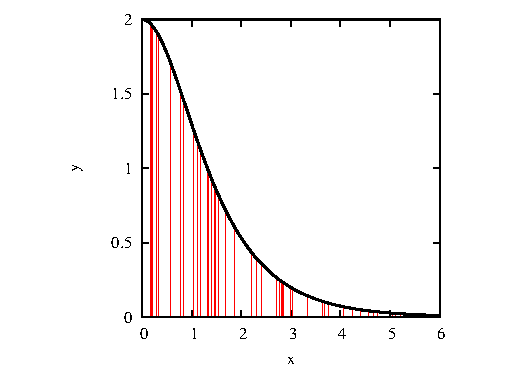
\includegraphics{image/coth-2.pdf}}
\end{frame}

\begin{frame}[t,fragile]{誤差の評価}
  \begin{itemize}
    \setlength{\itemsep}{1em}
  \item 関数 $f(x)/p(x)$ の分散
    \[
    s^2 = \int_0^c \Big(\frac{f(x)}{p(x)}\Big)^2 p(x) \, dx - \pi^2 = c \int_0^\infty f^2(x) \, dx - \pi^2 = 4c - \pi^2
    \]
  \item $c=20$ のとき $s^2 \simeq 70.1$
  \item 同じ試行回数 $M$ の時, 誤差は$\sqrt{70.1/116} = 0.77$ 倍
  \item もしくは $M$ を $116/70.1 = 1.65$ 倍したのと同じ効果
  \item 積分次元は低ければ低いほど良い
  \end{itemize}
\end{frame}

\begin{frame}[t,fragile]{次元の呪い(curse of dimensionality)}
  \begin{itemize}
    %\setlength{\itemsep}{1em}
  \item $n$次元超立方体(1辺の長さ 2, 体積 $2^n$)に対する$n$次元単位球の体積の割合
    \[
    q = \frac{\pi^{n/2} / \Gamma(\frac{n}{2}+1)}{2^n} \sim (\pi/n)^{n/2}
    \]
    $n=10$ で 0.2\%, $n=20$ で $10^{-8}$, $n=100$ で $10^{-70}$
  \item モンテカルロ積分で球の体積を計算しようとすると, 標準偏差に対する平均値の割合は指数関数的に小さい
    \[
    \frac{q}{\sqrt{q(1-q)}} \sim \sqrt{q}
    \]
  \item 次元が高くなるにつれて指数関数的に大きな $M$ が必要となる
  \item c.f. 通常の数値積分(台形公式等)でも同様
  \end{itemize}
\end{frame}

\begin{frame}[t,fragile]{重点的サンプリング}
  \begin{itemize}
    \setlength{\itemsep}{1em}
  \item (平均値が同じなら)被積分関数の分散が小さければ小さいほど良い (= 統計誤差が小さい)
  \item サンプリングの分布 $p(x)$ の形が $f(x)$ に近い程良い
  \item $f(x)$ の値が大きい所はより頻繁にサンプリング
  \item 重点的サンプリング (importance sampling)
  \end{itemize}
\end{frame}

\begin{frame}[t,fragile]{重点的サンプリング}
  \begin{itemize}
    \setlength{\itemsep}{1em}
  \item 積分への寄与が大きな箇所をより重点的にサンプリング
    \[
    p(x) = e^{-x}
    \]
    \begin{tabular}{|c|c|c|}
      \hline
      $M$ & 平均値 & 誤差 \\
      \hline
      100 & 3.06 & 0.06 \\
      10000 & 3.142 & 0.006 \\
      1000000 & 3.1412 & 0.0006 \\
      \hline
    \end{tabular}
  \end{itemize}
  \vspace*{-7em}
  \hspace*{17em}
  \resizebox{!}{.45\textheight}{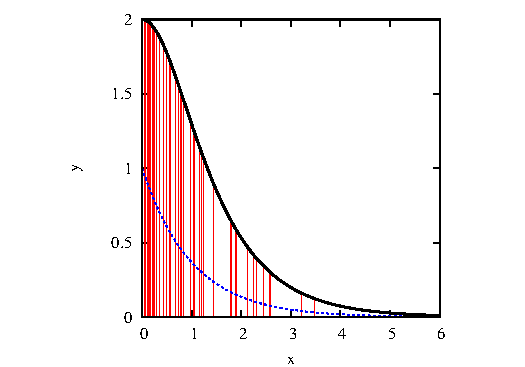
\includegraphics{image/coth-3.pdf}}
\end{frame}

\begin{frame}[t,fragile]{誤差のサンプル数依存性}
  \begin{itemize}
    \setlength{\itemsep}{1em}
  \item 関数 $f(x)/p(x)$ の分散
    \[
    s^2 = \int_0^c \Big(\frac{f(x)}{p(x)}\Big)^2 p(x) \, dx - \pi^2 \simeq 2(2+\pi) - \pi^2 = 0.414
    \]
  \item 同じ試行回数 $M$ の時, 誤差は

    $\sqrt{0.414/116} = 0.06 \mbox{倍}$

  \item もしくは $M$ を 280 倍したのと同じ
  \vspace*{-5em}
  \hspace*{15em}
  \resizebox{!}{.45\textheight}{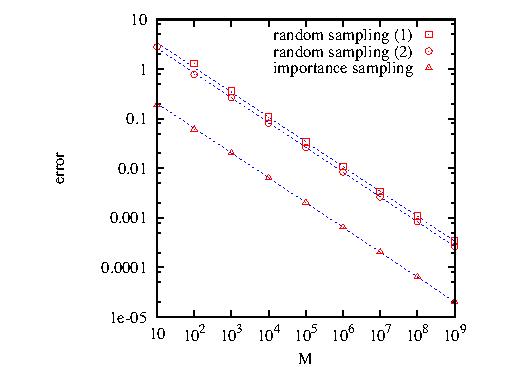
\includegraphics{image/sech-error.pdf}}
  \end{itemize}
\end{frame}

\begin{frame}[t,fragile]{理想的な重点的サンプリング?}
  \begin{itemize}
    \setlength{\itemsep}{1em}
  \item 理想的には $p(x)$ を $f(x)$ に比例するように取れば良い
  \item このとき $f(x) / p(x)$ は定数(分散 0) → 1回のサンプリングで厳密な結果が得られる???
  \item 実際には $p(x)$ が確率密度となるように規格化条件から定数 $c$ を決めておく必要あり
    \[
    \int p(x) \, dx = c \int f(x) \, dx = 1
    \]
  \item $c$ は今欲しい答そのもの!
  \end{itemize}
\end{frame}

% -*- coding: utf-8 -*-

\section{マルコフ連鎖モンテカルロ}

\begin{frame}[t,fragile]{統計物理における平衡状態}
  \begin{itemize}
    \setlength{\itemsep}{1em}
  \item Boltzmann分布 ($\beta \equiv 1/k_B T$)
    \[
    \pi(s) = \exp[-\beta {\cal H}(s)] \Big / \sum_s \exp[-\beta {\cal H}(s)]
    \]
  \item 物理量の期待値
    \[
    \langle A \rangle = \sum_s A(s) \exp[-\beta {\cal H}(s)] \Big/ \sum_s \exp[-\beta {\cal H}(s)]
    \]
  \item $\sum_s$は全ての状態に関する和 (系の体積に対して指数関数的に増加)
  \item 全ての状態について和をとるかわりに、Boltzmann重みが大きい(=$\cal H$が小さい)ところだけをモンテカルロ・サンプリング
  \end{itemize}
\end{frame}

%-*- coding:utf-8 -*-

\begin{frame}[t,fragile]{マルコフ連鎖モンテカルロ}
  \begin{itemize}
    %\setlength{\itemsep}{1em}
  \item 任意の多次元確率分布(今の場合はカノニカル分布)について、その分布したがうサンプル(状態)を生成する方法
    \begin{itemize}
    \item 直接カノニカル分布から独立したサンプリングをおこなうことは難しい
    \item 直前の状態からある確率にしたがって、次の状態を生成(マルコフ連鎖、Markov chain)
      \[
      \begin{split}
        &{\rm Pr}(X_{n+1}=s_j \,|\, X_0 = s_{i_0}, X_1 = s_{i_1}, \cdots, X_n = s_{i}) \\
        & \qquad = {\rm Pr}(X_{n+1}=s_j \,|\, X_n = s_{i}) = P_{i,j}
      \end{split}
      \]
    \item 長時間極限でカノニカル分布が達成されるように遷移確率(行列)$P_{i,j}$を選ぶ
      \[
      \lim_{n\rightarrow\infty}{\rm Pr}(X_n=s_j) \sim \pi_j = \exp[-\beta {\cal H}(s_j)]
      \]
    \end{itemize}
  \end{itemize}
\end{frame}

%-*- coding:utf-8 -*-

\begin{frame}[t,fragile]{遷移行列が満たすべき条件}
  \begin{itemize}
    % \setlength{\itemsep}{1em}
  \item 確率であるための条件: $0 \le P_{i,j} \le 1$
  \item 確率保存: $\sum_j P_{i,j} = 1$
  \item エルゴード性(ergodicity): \\
    ある整数$M$が存在し、$n \ge M$の全ての$n$で$(P^n)_{i,j} > 0$
  \item つりあいの条件(balance condition):
    \[ \sum_{i=1}^k \pi_i P_{i,j} = \pi_j \]
    カノニカル分布が固有値1の左固有ベクトル
  \end{itemize}
\end{frame}

\begin{frame}[t,fragile]{Perron-Frobeniusの定理}
  \begin{itemize}
    %\setlength{\itemsep}{1em}
  \item 正の正方行列$A$(すべての要素が正)について以下が成り立つ
    \begin{itemize}
      \item 他の全ての固有値よりも絶対値の大きな正の固有値$r$が存在する
      \item 固有値$r$は単純固有値である(縮退していない)
      \item 固有値$r$に対する右(左)固有ベクトル$v$ ($w$) は正のベクトルである
      \item 固有値 $r$ は $\displaystyle \min_i \sum_j a_{ij} \le r \le \max_i \sum_j a_{ij}$ を満たす
    \end{itemize}
  \item $A$が零の要素を持つ場合でも$A$が原始的(primitive = エルゴード的)である限り、上の結果は成り立つ
  \item 遷移行列は上の条件を満たす
    \begin{itemize}
    \item Boltzmann分布は絶対値最大の固有ベクトル
    \item 遷移行列を掛けていくとBoltzmann分布に収束
    \end{itemize}
  \end{itemize}
\end{frame}

\begin{frame}[t,fragile]{詳細つりあいの条件}
  \begin{itemize}
    \setlength{\itemsep}{1em}
  \item 実際には「つりあいの条件」よりもさらに厳しい「詳細つりあいの条件 (detailed balance condition)」を考えることが多い
    \[ \pi_i P_{i,j} = \pi_j P_{j,i} \]
  \item 両辺を $i$ について和をとると「つりあいの条件」に帰着する
  \item 「詳細つりあいの条件」は「つりあいの条件」の十分条件
  \end{itemize}
\end{frame}

%-*- coding:utf-8 -*-

\begin{frame}[t,fragile]{調和ポテンシャル中の古典粒子}
  \begin{itemize}
    %\setlength{\itemsep}{1em}
  \item ポテンシャルエネルギー
    \[ \hspace*{-4em} V(x) = x^2 \]
  \item カノニカル分布
    \[ \hspace*{-4em} P(x) = \frac{e^{-\beta V(x)}}{\int e^{-\beta V(x)} \, dx} \]
  \item 物理量の期待値
    \[ \hspace*{-4em} \langle x^2 \rangle = \frac{\int x^2 e^{-\beta V(x)} \, dx}{\int e^{-\beta V(x)} \, dx} \]
  \item 逆温度$\beta$が大きいと被積分関数の分散が非常に大きい $\Rightarrow$ 重点的サンプリング
  \end{itemize}
  \vspace*{-15em} \hfill
  \resizebox{4cm}{!}{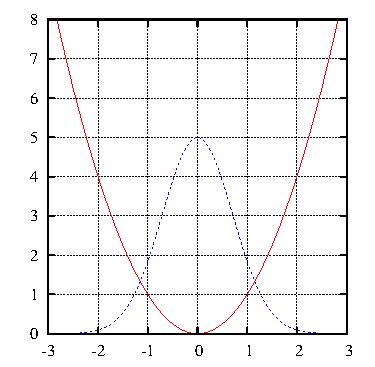
\includegraphics{image/harmonic.pdf}}
\end{frame}

%-*- coding:utf-8 -*-

\begin{frame}[t,fragile]{Metropolis法}
  \begin{itemize}
    %\setlength{\itemsep}{1em}
  \item 現在の配位$x$から、試行配位(trial configuration) $x'$を$x - \Delta \sim x + \Delta$の一様分布より選ぶ
  \item 確率$\min \Big( 1, \frac{e^{-\beta V(x')}}{e^{-\beta V(x)}} \Big)$で$x'$を採択(accept)。棄却(reject)された場合にはもとの$x$のまま
  \item 物理量の測定 (reject された場合にもカウントする)
  \item 採択確率(acceptance probability)は、$\frac{e^{-\beta V(x')}}{e^{-\beta V(x)}+e^{-\beta V(x')}}$でもよい
  \item 例: \href{https://github.com/todo-group/computer-experiments/blob/master/exercise/monte_carlo/harmonic.c}{harmonic.c}
  \end{itemize}
\end{frame}

\begin{frame}[t,fragile]{Metropolis法によるシミュレーション}
  \begin{itemize}
    \setlength{\itemsep}{1em}
  \item $\Delta = 0.1$
    
    \vspace*{-2em}\hfill \resizebox{9cm}{!}{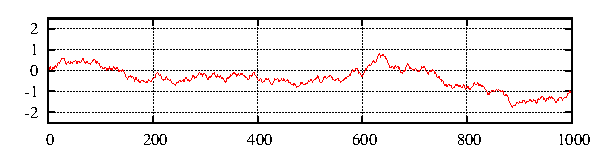
\includegraphics{image/series-001.pdf}}
  \item $\Delta = 1$
    
    \vspace*{-2em}\hfill \resizebox{9cm}{!}{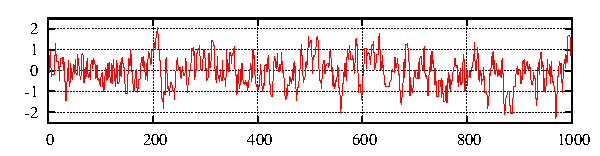
\includegraphics{image/series-010.pdf}}
  \item $\Delta = 10$
    
    \vspace*{-2em}\hfill \resizebox{9cm}{!}{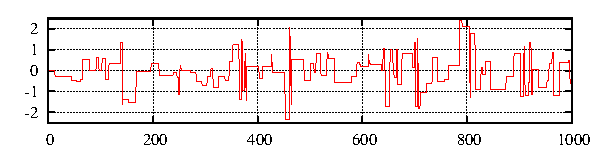
\includegraphics{image/series-100.pdf}}
  \end{itemize}
\end{frame}

%-*- coding:utf-8 -*-

\begin{frame}[t,fragile]{自己相関関数(autocorrelation function)}
  \begin{itemize}
    %\setlength{\itemsep}{1em}
  \item エルゴード性 + つりあい条件 ⇒ 原理的に正しいマルコフ連鎖モンテカルロ
  \item 実際には自己相関を考慮する必要あり
  \item 自己相関関数
    \[
    C(t) = \frac{\langle A_{i+t}A_i \rangle - \langle A \rangle^2}{\langle A^2 \rangle - \langle A \rangle^2} \sim \exp(-\frac{t}{\tau})
    \]
  \item $\tau$: 自己相関時間(autocorrelation time)
  \item 自己相関の影響により、統計的な「有効サンプル数」が減少
    \[
    M \rightarrow \frac{M}{1+2\tau}
    \]
  \end{itemize}
\end{frame}

\begin{frame}[t,fragile]{自己相関時間と統計誤差}
  \hspace*{4em} 自己相関時間 \hspace*{9em} 統計誤差

  \noindent\resizebox{0.49\textwidth}{!}{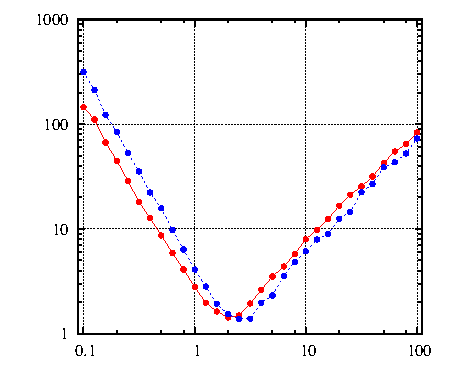
\includegraphics{image/autocorr.pdf}}
  \resizebox{0.49\textwidth}{!}{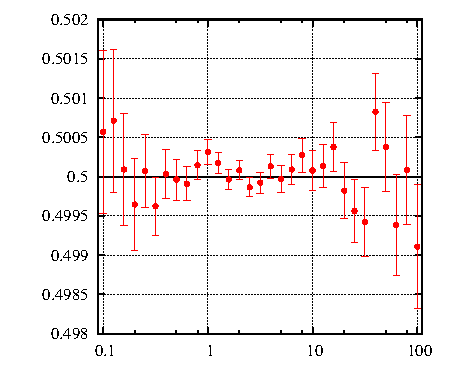
\includegraphics{image/error.pdf}}

  \hspace*{7em} $\Delta$ \hspace*{12em} $\Delta$
\end{frame}

\begin{frame}[t,fragile]{マルコフ連鎖モンテカルロ法}
  \begin{itemize}
    %\setlength{\itemsep}{1em}
  \item 統計誤差はサンプルの生の分散$s^2$とサンプル数$M$、自己相関時間$\tau$で決まる
    \[
    \sigma^2 \simeq \frac{s^2 (1+2\tau)}{M}
    \]
    \begin{itemize}
    \item 一度に大きく配位を動かそうとすると棄却率が増加 $\Rightarrow$ $\tau$が増加
    \item 動かす幅を小さくすると棄却率は高いが相関が消えない $\Rightarrow$ $\tau$が増加
    \item 非局所更新法、拡張アンサンブル法など様々な方法が使われている
    \end{itemize}
  \item 物理以外でも、Bayes推定や機械学習、社会現象のシミュレーションなど広く使われている
  \end{itemize}
\end{frame}

\begin{frame}[t,fragile]{イジング模型に対するモンテカルロ法}
  \begin{itemize}
    %\setlength{\itemsep}{1em}
  \item 更新の単位は一つのスピンとするのが一番自然
  \item メトロポリス法に必要なのは更新前後のエネルギー差だけなので、全エネルギーを計算しなおす必要なし
\begin{verbatim}
for (s = 0; s < num_sites; ++s) {
  delta = 0.0;
  for (j = 0; j < num_neighbors; ++j) {
    v = neighbor(s, j);
    delta += 2 * J * spin[s] * spin[v];
  }
  if (random() < exp(-beta * delta))
    spin[s] = -1 * spin[s];
}  
\end{verbatim}
  \end{itemize}
\end{frame}

\begin{frame}[t,fragile]{物理量の計算}
  \begin{itemize}
    %\setlength{\itemsep}{1em}
  \item 内部エネルギー$E$
    \begin{itemize}
    \item 初期状態のスピンを全て上向き(1)に取ると$E=-J \times \text{ボンド数}$
    \item モンテカルロステップ毎にエネルギーの変化分を計算しているので、採択された場合にはその値を足し込む
    \end{itemize}
  \item 比熱$C$: 内部エネルギーのゆらぎから計算できる
    \[
    C = \frac{1}{N} \frac{\partial E}{\partial T} = \frac{1}{NT^2} (\langle E^2 \rangle - \langle E \rangle^2)
    \]
  \item 磁化$m$: スピンの値の平均値 $m = \frac{1}{N} \sum_i \sigma_i$
    \begin{itemize}
    \item 外部磁場がない場合、対称性から$m$の長時間平均は厳密には零になる
    \item 熱力学極限では対称性が自発的に破れて、低温で有限の$m$
    \item シミュレーションでは$m$ではなく$m^2$を見るとよい
    \end{itemize}
  \end{itemize}
\end{frame}

%-*- coding:utf-8 -*-

\begin{frame}[t,fragile]{モンテカルロステップの設定}
  \begin{itemize}
    %\setlength{\itemsep}{1em}
  \item 全てのスピンについて一通り更新を試すのを、1モンテカルロステップと数える
  \item どれくらいのモンテカルロステップが必要かは、あらかじめは分からない
  \item 典型的には、$10^4$---$10^6$程度にとることが多い
  \item 熱平衡化 (thermalization)
    \begin{itemize}
    \item 初期配位依存性を取り除くため、モンテカルロステップの最初の部分は捨てる(burn-in time)
    \item 典型的には、全体の1割程度を捨てることが多い
    \end{itemize}
  \end{itemize}
\end{frame}



\end{document}
